% !TeX root = ../main.tex
% Add the above to each chapter to make compiling the PDF easier in some editors.

\chapter{Literature Review}\label{chapter:literature_review}

\section{Geo-based Content Sharing}
In typical networks (such as social networking etc.), the content is shared among users irrespective of their geographic location. There are a number of advantages to this such as:

\begin{itemize}
  \item High availablity
  \item Reliability
  \item large amount of content. 
\end{itemize}

However, there are some disadvantages with such networks such as:

\begin{itemize}
  \item A connected network is needed for the services to work, so in case the connectivity is lost, normally the content is also gone.
  \item The system/network is prone to censorship
\end{itemize}

Geo-based content sharing has been introduced to make the information/content more customized based on the user location such as chatting with people nearby, posting in a local message board etc. There are two types of networks used for Geobased content sharing: \emph{Connected Systems/Networks} and \emph{Peer to Peer Systems/Networks}.

\subsection{Connected Systems/Networks}
\textit{TODO: Write about a few connected networks apps}

\subsection{Peer to Peer Systems/Networks}
Peer to Peer Networks don't relay on the network infrastructure to relay information, so they can work even when there is No server/central controller or no pre-determined path between the sender and reciever. A key property of such systems is that they do not rely on infrastructure nodes or cloud services to ensure data availability but rather replicate content items within the anchor zone among mobile nodes in a device-to-device (peer-to-peer) fashion. While this operation does not require infrastructure network access—and thus limits dependencies as well as vulnerability to third party actions such as traceability or censorship—it comes at the cost of unpredictability: there is no guarantee that content “posted” to an anchor zone will remain available. We refer to this property as best-effort (probabilistic) content sharing \cite{geo-based-content-sharing}.

Below are the four different systems utilizing this methodology:
\begin{itemize}
  \item Hovering Information
  \item Locus
  \item Ad Loc
  \item Floating Content
\end{itemize}

\subsubsection{Hovering Information \cite{Castro2009}} 
Hovering information is a concept characterising self-organising information responsible to find its own storage on top of a highly dynamic set of mobile devices. The main requirement of a single piece of hovering information is to keep itself stored at some specified location, which we call the anchor location, despite the unreliability of the device on which it is stored. Whenever the mobile device, on which the hovering information is currently stored, leaves the area around the specified storage location, the information has to hop - ”hover” - to another device.
\subsubsection{Locus \cite{Thompson:2010:LLD:1859934.1859945}} 
Locus, a location-based data overlay for DTNs. Locus keeps objects at specific physical locations in the network using whatever devices currently are nearby. Nodes copy objects between themselves to maintain the locality of data. Location utility functions prioritize objects for replication and enable location-based forwarding of data look-ups. As a first-of-its-kind application, Locus is compared against other possible replication policies and shown to achieve query success rates nearly 4 times higher than other approaches.
\subsubsection{Ad Loc} 
Ad Loc is a platform that enable users to tie persistent virtual notes to physical locations without the need for embedded infrastructure in the environment or access to the internet \cite{Corbett2006ADL}.
\subsubsection {Floating Content}
Floating content is an ephemeral content sharing service, solely dependent on the mobile devices in the vicinity using principles of opportunistic networking. The net result is a best effort service for floating content in which: 1) information dissemination is geographically limited; 2) the lifetime and spreading of information depend on interested nodes being available; 3) traffic can only be created and caused locally; and 4) content can only be added, but not deleted \cite{floating-content}. Floating Content is discussed in more details \hyperref[section:floating-content]{\emph{later in the chapter}}.

\newpage
\section{The ONE Simulator}
\subsection{Introduction}
The ONE is an Opportunistic Network Environment simulator \cite{the-one} which provides a powerful tool for generating mobility traces, running DTN messaging simulations with different routing protocols, and visualizing both simulations interactively in real-time and results after their completion \cite{the-one-ari}.

Delay-tolerant Networking (DTN) enables communication in sparse mobile ad-hoc networks and other challenged environments where traditional networking fails and new routing and application protocols are required. Past experience with DTN routing and application protocols has shown that their performance is highly dependent on the underlying mobility and node characteristics \cite{keranen-theone}. The basic idea behind DTN is to communicate data/messages from the source to the destination without having complete network connectivity. The path from the source to the destination is unknown due to the unconnected nature of the network. In such networks, each node store the messages it receive and forward it to the next node it comes in contact with. The message may or may not reach its final destination.

The ONE simulator was originally developed in Aalto University in the SINDTN \cite{sindtn} and CATDTN projects supported by Nokia Research Center (Finland). It is now maintained in by Aalto Univerity in cooperation with Technical University of Munich.\newline

The ONE Simulator has the following capabilities:
\begin{itemize}
  \item Message Generation at different intervals.
  \item Node Movement using different movement models such as Random Walk, Map based movement etc.
  \item Routing messages between nodes using different types of routers such as Epidemic Router, First Contact Router etc.
  \item Graphical User Interface (GUI) for visualizing nodes movement, message creation and message passing in real time.
  \item Report Generation for different purposes such as Message Delivery Report etc.
  \item Batch mode where the app can be run without a GUI.
\end{itemize}

\begin{figure}[h]
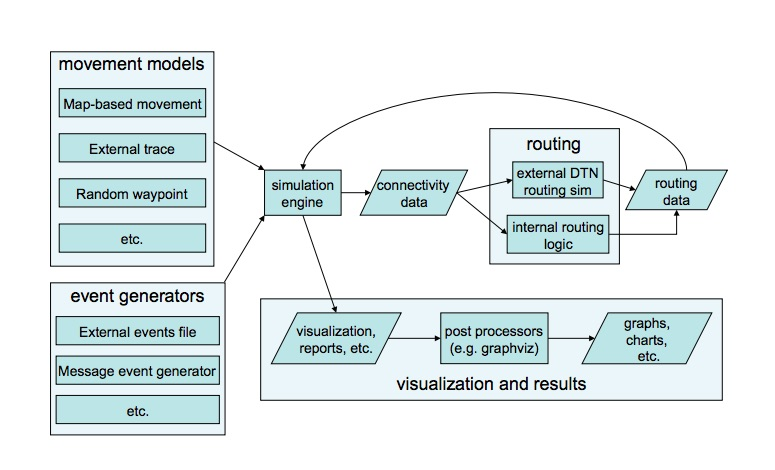
\includegraphics[scale=0.5]{./figures/one}
\caption{Overview of the ONE simulation Environment \cite{keranen-theone}}
\end{figure}

\subsection{Components}
\subsubsection{Host Group}
Host Groups represents a collection of hosts with the same configuration such as Movement Model etc. In other words, similar nodes are grouped in a Host Group. Theoretically, each host group must have different configuration from the other host groups. All the host groups can also share configuration (such as number of hosts etc.) which are defined under "Group" namespace. However, configuration inside the specific host group takes precedence over the global "Group" namespace.
\subsubsection{Movement Models}
Movement Models dictate the node movements in the simulation. A number of Movement Models come packaged with the ONE simulator such as \textit{Map based Movement}, \textit{Shortest Path Map based Movement}, \textit{Random Waypoint}, \textit{External Movement} and \textit{Stationary Movement}. \textit{MapBased Movement} have further types of movements such as \textit{Car Movement} and \textit{Map Route Movement} etc.
\subsubsection{Routing}
Routing Module is responsible for handling the transfer (routing) of messages between hosts. ONE simulator one passive and a number of active routers. Passive router is used for interacting with other DTNs or dummy nodes. The active routers implements the well known routing algorithms for DTN such as \textit{Epidemic}, \textit{Spray and Wait}, \textit{First Contact}, \textit{Direct Delivery}, \textit{Prophet}, \textit{Prophet V2}, \textit{Life}, \textit{Wave}, \textit{MaxProp} and \textit{Floating Content}.

\subsection{Compilation}
ONE can be compiled from the source code using both Command Line and Eclipse.

\subsubsection{Command Line}
  The ONE source contains \textit{compile.sh} and \textit{compile.bat} for compilation on the Linux/Unix and Windows Platform respectively.

\subsubsection{Eclipse}
The project has three main dependencies (\textit{DTNConsoleConnection.jar}, \textit{ECLA.jar} and \textit{JUnit}) that need to be added. 
\begin{itemize}
  \item Import the Project into Eclipse
  \item Right Click on Project -> Properties -> Java Build Path -> Libraries.
  \item Click on Add Jar -> Navigate to lib -> Select \textit{DTNConsoleConnection.jar} -> OK.
  \item Repeat for \textit{ECLA.jar}
  \item Click on Add Library -> JUnit -> (Optionally) Select JUnit version -> Finish.
\end{itemize}


\subsection{Running}
Just like Compilation, ONE can be run from both Command Line and Eclipse.

\subsubsection{Command Line}
\begin{lstlisting}[language=bash]
./one.sh [-b repetitionCount] [configuration-files]
./one.bat [-b repetitionCount] [configuration-files]
\end{lstlisting}

\textbf{-b} is an optional parameter. Start the ONE simulator in batch (non-UI) mode. \textit{repetitionCount} specifies the number of times the simulations needs to repeat. If not defined, the ONE simulator starts in UI mode.\newline
\textbf{configuration-files} is an optional parameters, where you can specify a number of configuration files separated by space. The simulation parameters are read from these files. Files specified later override values in the earlier config files.\newline

\subsubsection{Eclipse}
By default, Eclipse launches the ONE simulator in UI mode. However, we can launch the simulator in batch mode and provide configuration files as well.
\begin{itemize}
  \item Click on Run Menu -> Run Configurations...
  \item Click on DTNSim in the left pan -> Click on Arguments tab in the right pane
  \item Specify the arguments under Program arguments the same way as you would do for Command Line.
  \item Click on Apply -> Run.
\end{itemize}

\subsection{Configuration}
\label{one:configuration}
One of the amazing features of ONE is that there is no need for changing the code and recompilation if need to change any configuration (such as changing the number of hosts, changing the movement models etc.). All of these can be done in the configuration files which are ordinary text files. By default, the ONE simulator uses \textbf{default\_settings.txt} configuration file. However, additional configuration files can also be passed.

Configuration files contain key-value pairs. Syntax for most of these pairs is:
\begin{lstlisting}[language=bash]
Namespace.key = value
\end{lstlisting}

Both \textit{Namespace} and \textit{key} follow the camelCase and are case sensitive. \textit{value} can be numeric, boolean, strings, comma-separated values, value filling and reference to other files. Numeric values can also use the suffixes \textit{k} for Kilo, \textit{M} for Mega and \textit{G} for Giga. 

\subsubsection{Value Filling} 
Value Filling is used to dynamically fill the value during run-time. The main purpose is to use the value of a variable during run-time. To use value-filling, put the key name as value surrounded by %% such as %%keyName%%. Below is an example:
\begin{lstlisting}[language=bash]
MovementModel.warmup = %%Reports.warmup%%
\end{lstlisting}
\subsubsection{Run Indexing} 
What happens if we want to run the simulations for different configurations such as a different routing protocol for each run. One solution would be to create different configurations and write a script passing the desired configuration for each run. However, it is not a maintainable solution if we have a different number of permutations (changing 3 values each for two different parameters). ONE simulator solves this problem by using Run Indexing. Run indexing allows us to change configuration during run-time by providing the same configuration file;  containing a set of semi-colon seprated values surrounded by braces ([]) for the deisred key(s).

\begin{lstlisting}[language=bash]
Reports.warmup = [0; 100; 200; 300]
\end{lstlisting}

In the above example, the first run will use the value 0, next one will use the value 100 and so on. In case the values are less than the total number of simulations, the indexes wrap around (loops back to the start of the array when there is no further item to read).
\newpage
\section{Floating Content}
\label{section:floating-content}
Floating content is an ephemeral content sharing service, solely dependent on the mobile devices in the vicinity using principles of opportunistic networking. The net result is a best effort service for floating content in which: 1) information dissemination is geographically limited; 2) the lifetime and spreading of information depend on interested nodes being available; 3) traffic can only be created and caused locally; and 4) content can only be added, but not deleted \cite{floating-content}.

In Floating Content, a message (a text message, an image, etc.) deemed to be of interest to other people at a certain area is tagged with geographical coordinates of that area. This area is referred to as the anchor-zone of the message \cite{floating-content-1}. Each message has two main properties namely \textit{Center} and \textit{Availability/anchor zone}. For the sake of simplicity, the anchor zone is defined as a circle with a radius. In short, floating messages can be relayed to other nodes inside the anchor zone. Every time a copy of the message is made, the anchor zone properties are copied to make sure that the copied message has the same anchor zone as the original message.

Whenever a message is generated, it is assigned an anchor zone (identified by a radius and the node's current location). The message is transferred to other nodes in the anchor zone. Whenever a node moves out of the anchor zone, it may delete its copy of the message or keep it until first interaction with another node depending on the configuration.
\begin{figure}[h]
\centering
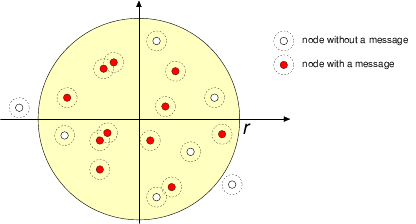
\includegraphics{./figures/anchor-zone}
\caption{Floating-Content and its anchor zone \cite{floating-content}}
\end{figure}
\newpage
\subsection{Floating Content and ONE Simulator}
Before continuing the discussion on Floating Content and its implementation in the ONE simulator, let us introduce a few concepts.
\begin{center}
    \captionof{table}{Floating Content: Imporant Concepts} \label{tab:title} 
    \begin{tabular}{ | l | p{11cm} |}
    \hline
    \textbf{Concept} & \textbf{Detail} \\ \hline
    \textit{interval} & minimum time between generation of two messages by the same node. \\ \hline
    \textit{radius (r)} & the replication range for floating message.  \\ \hline
    \textit{anchor (a)} & the availability range of the floating message. \\ \hline
    \textit{time to live (ttl)} & The message life (seconds) for the floating message. \\ \hline
    \textit{size} & The size of the floating message. \\ \hline
    \textit{replicationPolicy} & dictates how floating messages are replicated when the node comes in contact with another node. \\ \hline
    \textit{deletionPolicy} & dictates when floating messages are deleted. \\ \hline
    \end{tabular}
\end{center}
\begin{center}
    \captionof{table}{Floating Content: Replication Policies} \label{tab:title} 
    \begin{tabular}{ | l | p{8cm} |}
    \hline
    \textbf{Replication Policy} & \textbf{Detail} \\ \hline
    \textit{first in first out (fifo)} & messages are replicated in the order they are found in the buffer. This is the default replication policy.\\ \hline
    \textit{random shuffle (rnd)} & Shuffle and select messages randomly for replication. \\ \hline
    \textit{smallest anchor zone first (saf)} & messages with the smallest anchor zone are replicated first.  \\ \hline
    \textit{smallest cylinder (radius) first (svf)} & messages with the smallest cylinder \textit{(anchor * message size)} are replicated first. \\ \hline
    \textit{smallest cylinder (area) first (svf2)} & messages with the smallest cylinder \textit{(anchor * anchor * message size)} are replicated first. \\ \hline
    \textit{smallest total (radius) first (stf)} & messages with the smallest total \textit{(anchor * ttl * message size)} are replicated first. \\ \hline
    \textit{smallest total (area) first (stf2)} & messages with the smallest total \textit{(anchor * anchor * ttl * message size)} are replicated first. \\ \hline

    \end{tabular}
\end{center}
\newpage
\begin{center}
    \captionof{table}{Floating Content: Deletion Policies} \label{tab:title} 
    \begin{tabular}{ | l | p{11cm} |}
    \hline
    \textbf{Deletion Policy} & \textbf{Detail} \\ \hline
    \textit{Encounter} & the message is deleted outside the anchor zone on first encounter with another node. The advantage/use case is that the node still cariies the message if it leaves the anchor zone for a short period of time (and does not enouncter another node during that period). It is the default policy in ONE Simulator. \\ \hline
    \textit{Immediate} & the message is deleted as soon as the node leaves the anchor zone. \\ \hline
    \end{tabular}
\end{center}

\subsubsection{Components}
The ONE Simulator has two main components for dealing with Floating Content which are \textit{FloatingApplication} and \textit{FloatingContentRouter}.

\begin{itemize}
\item \textit{FloatingApplication} is responsible for generation of the messages with the floating content parameters (such as anchor, ttl etc.). FloatingApplication can be associated with any Host Group (or all the Host Groups) using the configuration file(s). 
\item \textit{FloatingContentRouter} is responsible for all the routing related functionalities for the floating messages. It takes care of replication, deletion (and dropping) and prioritization of message. Replication and Deletion is performed as per the Replication and Deletion policies. Different parameters of the FloatingContentRouter can be set in configuration file(s).
\end{itemize}


\subsubsection{Configuration}
As mentioned in \hyperref[one:configuration]{\emph{Configuration of ONE Simulator}}, all the configurations need to be provided as configuration files containing key-value pairs. Below are some examples for setting configuration for the floating content.

\begin{lstlisting}[language=bash]
# Setting the Group (global) router to FloatingContentRouter
Group.router = FloatingContentRouter


# FloatingContent Router with first in first out replication and immediate deletion
FloatingContentRouter.seed = [0; 1; 2; 3; 4; 5; 6; 7; 8; 9 ]   # run-indexed seed for random number generator
FloatingContentRouter.replicationPolicy = fifo
FloatingContentRouter.deletionPolicy = immediate


#Floating App configuration
floatingApp.seed = [0; 1; 2; 3; 4; 5; 6; 7; 8; 9 ]

floatingApp.type = FloatingApplication
floatingApp.startTime = 0
floatingApp.interval = 1800
floatingApp.ttl = 300
floatingApp.destination = 0
floatingApp.messageSize = 5k
floatingApp.anchor = 200


# Assigning Floating app to all Groups
Group.nrofApplications = 1
Group.application1 = floatingApp


# Assigning Floating app to only 1 Group
Group1.nrofApplications = 1
Group1.application1 = floatingApp

\end{lstlisting}